% =========================================================================
% CHAPTER 6
% =========================================================================

\chapter{Diskussion}

\section{Vorteile der Middleware Implementierung und der gewählten Technologien}
Die Vorteile der entstandenen Middleware können eingeteilt werden in diejenigen, die durch die Requirements entstehen, und denen, die durch das Software Design entstehen. Die bereits in (3) beschriebenen Eigenschaften leichtgewichtig, große Bandbreite an Betriebssystemen, Abbrechbarkeit, Progress Anzeige und Feedback über die korrekte Terminierung aller Worker Aufgaben resultieren aus den Requirements.
Das Design der Implementierung hat weitere Vorteile ergeben, die noch nicht näher beschrieben wurden. Timeouts für alle asynchronen Operationen, kein Deployment und Erweiterbarkeit.

Jeder Job kann mit einem Timeout versehen werden. Netzwerkprogrammierung erfordert häufig die Berücksichtigung von Timeouts, meist im Zusammenhang mit asynchronen Vorgängen. Die Vereinigung dieser beiden Features in einer Klasse ermöglicht eine kompakte Implementierung der Requirments mit weniger als 1000 Zeilen JavaScript. Timeouts finden auch bei lokalen asynchronen Operationen Anwendung. Man kann zwar Hardware Fehler ausschließen, aber Implementierungsfehler, wie zum Beispiel das fehlende Schließen eines Jobs wird nicht erkannt. Eine solche fehlerhafte Implementierung wird ein Timeout auslösen, was die Fehlersuche erleichtert.

Der Anwender ist in der Lage, beliebige Verteilungsstrategien mit Hilfe von Jobscripts zu definieren, ohne einen Deployment Process auszuführen. Das Skript wird während der Ausführung an die entsprechenden Geräte verteilt - dies könnte auch als Deployment zur Runtime gesehen werden - jedenfalls geschieht es automatisch.

Mit der Hilfe der Job.delegate Funktion können Abhängigkeiten zwischen den Jobs definiert werden. Die Middleware kann so zur Laufzeit einen JobTree aufbauen, der zu Debugging und Usability Zwecken verwendet werden kann. Zum Beispiel ist im Fehlerfall daraus ersichtlich, auf welchem Gerät der Fehler stattgefunden hat. Auch Performance-Analysen und Ablaufvisualisierungen sind damit möglich.

Das Konzept ist auf einer tiefen Ebene im Schichtenmodell angesiedelt. Erweiterungen hin zu einem Map Reduce- oder einem Apache Spark ähnlichem System erfordern keine Änderungen, sondern eine Erweiterung um eine Schicht darüber.


\section{RootJob Events und UI}
Die onUpdate und onReturn Events der RootJobs sind nicht implementiert und können für die Anbindung des UI verwendet werden. Die Anbindung ist sehr einfach, da die beiden Events alle durch das Netzwerk veruhrsachten UI Updates abdecken.
Das gilt für das Anzeigen von Ergebnissen genauso wie für die Anzeige des Progress, Enablen/Disable Events und Fehlermeldungen - egal, ob lokal oder remote.

Cancel Implementierungen sind vereinfacht durch das triviale Auslösen eines Abbruchs mit einem Funktionsaufruf und die vom System erkannten Fehlern, welche durch Race Conditions verursacht werden. Diese können ebenfalls im UI dargestellt werden, indem im onReturn Event auf die Zustände der SubJobs geachtet wird.




\section{Nachteile der Middleware Implementierung}
Nachteile, die durch fehlende Implementierung entstehen und in Zukunft erweitert werden können, sind ein primitiver Scheduler (sihe 6.3) und eine begrenzte Auswahl von Workflow Logiken.

Nachteile, die aus dem gewählten Softwaredesing resultiere,n sind mögliche Überlastung des Servers bei schlechten JobScript Implementierungen (siehe 6.4), und ein vollständiges außer Acht lassen von Security Maßnahmen. Duch das Übertragen der Scripts werden Angriffsmöglichkeiten eröffnet. Ein möglicher Lösugsansatz wären abgesicherte Sandboxes am Server und den Workern, wobei bedacht werden muss, dass das Starten von Prozessen ein gewünschtes Feature ist.
Die Verwendung von Secure Websockets, einer Benutzeranmeldung am Client und eine Assoziation der Websocket Verbindung mit einem Benutzer am Server wäre ebenso denkbar. Dabei ist jedoch zu beachten, dass für jeden Benutzer des Webservers auch ein Benutzer im Betriebssystem angelegt werden muss.

Eine genaue Evaluierung möglicher Security Konzepte könnte in einer zukünftigen Arbeit erfolgen.




\section{WorkerJob mit längster Laufzeit am Ende der Pool Queue}
Folgendes Script führt 10 WorkerJobs mit zufälliger Laufzeit zwischen einer und 15 Sekunden in einem Pool von drei Workern aus.
\begin{figure}[H]
  \centering
    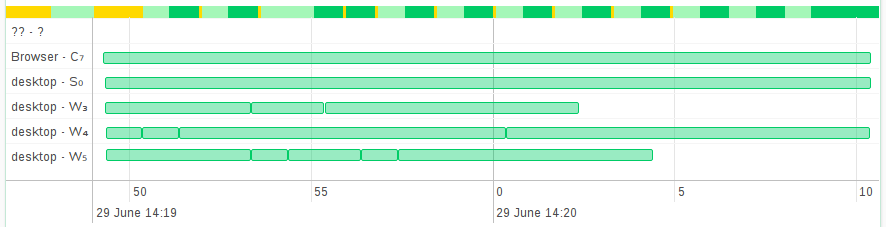
\includegraphics[width=\textwidth]{gant}
    \caption{Flower one.}
\end{figure}
\noindent Abbildung XY zeigt, dass zwei von drei Workern mehr als ein Viertel der gesamten Laufzeit idle waren, also das System weniger als 84% ausgelastet war. Ungünsige Konstellationen können eine noch weitaus schlechtere Auslastung zur Folge haben. Bei unrgelmäßigen WorkerJob Laufzeiten können komplexere Scheduler für eine bessere Auslastung sorgen.

Kurz nachdem der letzte WorkerJob auf W4 terminiert, terminiert der ServerJob S0 und danach der Rootjob am Client C7. Die Verzögerung, bestehend aus Netzwerklatenz und Verarbeitungszeit der return Transition, ist minimal - in dieser Darstellung kaum sichtbar.





\section{Server/Client Überlastung}
Folgendes Script führt 20 ‘leere’ WorkerJobs, dass heißt sie terminieren direkt nach dem Start, in einem Pool von drei Workers aus.
\begin{figure}[H]
  \centering
    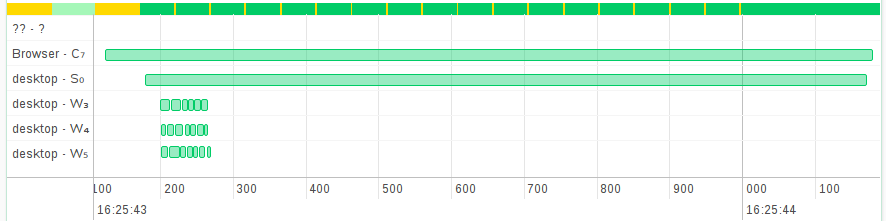
\includegraphics[width=\textwidth]{gant2}
    \caption{Flower one.}
\end{figure}
\noindent Abbildung XY zeigt eine Überlastung des Clients oder Servers, erkennbar an der großen Zeitspanne zwischen dem Ende des letzten WorkeJobs und dem Ende des ServerJobs. Diese Verzögerung setzt sich zusammen aus Netzwerklatenz und onReturn Transition Verarbeitung, jeweils für den Server und Client - auf Server und Client, weil der auf S0 ausgeführte Job auf C7 erstellt wurde und die Joblaufzeit am auftraggebenden Gerät gemessen wird. Ob die Verzögerung auf dem Server oder Client entstanden ist, kann anhand dieses Diagramms nicht bestimmt werden. Eine Erweiterung der Visualisierung, die die Queueläge zeigt, würde die Identifizierung des überlasteten Geräts ermöglichen.




\section{Conclusion and Future Work}
Es wurden JobScripts für zwei Network Overlays implementiert, Client Server und HCSNO mit einer Worker Ebene. Kapitel 7 zeigt die Skalierbarkeit des HCSNO für verschiedene Algorithmen. Die Skalierbarkeit ist derzeit durch Serverüberlastungen begrenzt, die auftreten, wenn zu viele Worker an den Server senden. Eine größere Anzahl von Workern ist nur möglich, wenn sie nicht alle mit einem Server verbunden sind. Ein hierarchisches Netzwerk mit mehren Ebenen von Server Nodes könnte eine Laufzeit  T(n) = ld(n) erreichen, wobei n die Gesamtanzahl der Worker ist.

Für diese Overlays wurden jeweils mehrere Test Scripts mit geringem Zeitaufwand  implementiert. Das Konzept könnte auch Anwendung bei der Implementierung von Prototypen finden. Die Network Overlay Struktur ist vorerst aber noch statisch zur Runtime und eine Änderung würde die Anpassung von Kernkomponenten erfodern. Eine Erweiterung um ein P2P Network Overlay würde einen interessanten Raum für Experimente schaffen.

Derzeit enthält der Webclient mehrere Visualisierungen: den Workflow Graph zu jedem Run eines Scripts, einen Gant Chart, der die Laufzeiten aller Jobs zeigt, sowie eine vereinfachte Darstellung des Netzwerks. Sie alle visualisieren dasselbe Model, den JobTree. Für dieses Model könnten noch weitere Visualisierungen geschaffen werden, die bei Debugging und Performance Analysen helfen würden.

Das Job API muss noch weiter vereinfacht werden. Eine Trennung des Jobs in zwei Komponenten, Future und Promise nach (baker1977incremental), scheint sinnvoll.
